\documentclass[10pt]{article}
\usepackage[margin=1in]{geometry}
\usepackage{graphicx}
\usepackage{booktabs}
\usepackage{hyperref}
\usepackage{listings}
\usepackage{xcolor}
\usepackage{caption}
\usepackage{subcaption}
\usepackage{setspace}
\usepackage{float}
\usepackage{fontspec}
\setmainfont{Latin Modern Roman}
\setsansfont{Latin Modern Sans}
\setmonofont{Latin Modern Mono}

\lstset{
  basicstyle=\small\ttfamily,
  breaklines=true,
  language=Python,
  frame=single,
  numbers=none
}

\title{\textbf{ML Compiler Opt: Training Loop Optimizations} \\
\large CPEG/ELEG652 Final Project Report}

\author{Andrew Kallai}
\date{May 6, 2026}

\begin{document}

\maketitle

\begin{abstract}
This report describes the optimization of the training loop in Google's MLGO (Machine Learning Guided Optimization) framework, which uses reinforcement learning to train compiler heuristics for LLVM. The project focused on improving the data pipeline, enabling XLA JIT compilation, and tuning hyperparameters for the Proximal Policy Optimization (PPO) training loop used to train inlining-for-size policies. Over three commits, the training iteration time was reduced and the system's observability was improved with performance counters and profiling integration.
\end{abstract}

\section{Application}

\subsection{Science Perspective}

MLGO \cite{mlgo2021} is a framework developed by Google to replace hand-crafted compiler heuristics in LLVM with machine-learned models. The core idea is to frame compiler optimization decisions---such as whether to inline a function---as a reinforcement learning (RL) problem. At each compilation decision point, an agent observes features of the current code (function size, call frequency, loop structure, etc.) and selects an action (inline or not). The reward is measured after compilation is complete, typically as the size of the generated binary (for inlining-for-size) or runtime performance (for register allocation).

The training process uses Proximal Policy Optimization (PPO), a policy gradient method. The workflow proceeds in iterations: (1) \textbf{Data collection}: the current policy is used to compile a corpus of modules (here, from the Fuchsia operating system), collecting trajectory data (state, action, reward) for each compilation decision; (2) \textbf{Training}: the collected trajectories are used to update the policy network via gradient descent. This alternating collect-train cycle repeats for many iterations.

The inlining-for-size task has practical importance: reducing binary size is critical for embedded systems, mobile devices, and operating system kernels. Prior work \cite{mlgo2021} demonstrated up to 7\% size reduction over LLVM's -Oz mode using MLGO-trained policies.

\subsection{Computer Science Perspective}

The \texttt{ml-compiler-opt} repository is written in Python (approximately 5,600 lines across 140 Python files), with heavy use of TensorFlow for neural network model definition, training, and inference. Key components include:

\begin{itemize}
    \item \textbf{Data collection}: parallel compilation of LLVM IR modules using subprocess workers
    \item \textbf{Data pipeline}: \texttt{tf.data.Dataset}-based pipeline for reading, parsing, shuffling, and batching trajectory data
    \item \textbf{Training loop}: PPO agent training implemented in TensorFlow with custom training steps
    \item \textbf{Configuration}: gin-config based hyperparameter management
\end{itemize}

The application was evaluated using the Fuchsia operating system codebase as the training corpus, with LLVM built from source with MLGO support. Training runs were executed on a Slurm cluster (node \texttt{odyssey}) with 64 parallel workers for compilation. A single training run (100 iterations, 16 modules per iteration) takes approximately 3--10 minutes depending on configuration, with the majority of time spent in LLVM compilation during data collection.

This project modified 11 files, adding 185 lines and removing 204 lines across three commits:

\begin{table}[H]
\centering
\caption{Summary of Commits}
\begin{tabular}{lrr}
\toprule
Commit & Files Changed & Net Lines \\
\midrule
Commit 1: Data Pipeline & 10 & $+151/-202$ \\
Commit 2: XLA JIT + Perf Counters & 4 & $+39/-6$ \\
Commit 3: XLA Flags Fix & 1 & $+1/-2$ \\
\midrule
Total & 11 (unique) & $+185/-204$ \\
\bottomrule
\end{tabular}
\end{table}

\section{Project Objective and Execution}

The objective of this project was to improve the throughput and observability of the MLGO PPO training loop. The original training loop suffered from several inefficiencies: excessive thread pool overhead in data collection, significant TensorFlow op dispatch overhead in the data pipeline, and single-threaded execution of matrix operations during training. Additionally, there was no instrumentation to measure where time was being spent.

\subsection{Commit 1: Data Pipeline Optimization}

The original data pipeline architecture used \texttt{concurrent.futures.ThreadPoolExecutor} to prefetch compilation modules asynchronously. While this seemed like a reasonable approach, it introduced excessive thread management overhead---the thread pool was created and destroyed each iteration, and the asynchronous future resolution added latency. Profiling revealed that \texttt{Iterator::Root::Prefetch} consumed approximately 18\% of host CPU time.

The changes made:

\begin{enumerate}
    \item \textbf{Removed \texttt{concurrent.futures} prefetching}: Replaced asynchronous module prefetch with synchronous \texttt{corpus.load\_module\_spec} calls in \texttt{local\_data\_collector.py}. This eliminated thread pool creation/destruction overhead and simplified the control flow.
    \item \textbf{Removed inter-iteration \texttt{\_reset\_workers} future}: The original code scheduled a deferred cleanup future between collect/train cycles, adding unnecessary complexity and potential synchronization delays.
    \item \textbf{\texttt{tf.data.Dataset} replacement with Python generator}: The most impactful change. The original pipeline used \texttt{tf.data.Dataset.from\_tensor\_slices()} with \texttt{.cache()}, \texttt{.repeat()}, and \texttt{.prefetch(AUTOTUNE)} operations. This incurred TensorFlow op dispatch overhead for every batch. The replacement uses a pure Python generator (\texttt{\_batched\_generator}) that eagerly parses serialized trajectories using \texttt{tf.constant()}, concatenates all frames, then slices them into \texttt{[B, T]} batches. The generator cycles infinitely via index reset rather than \texttt{.repeat()}.
    \item \textbf{Reduced shuffle/buffer sizes}: The file-based dataset path (used as fallback) had its shuffle and buffer sizes drastically reduced (e.g., \texttt{files\_buffer\_size}: 100$\rightarrow$2, \texttt{shuffle\_buffer\_size}: 1024$\rightarrow$2) since with the in-memory generator path as primary data source, large buffers were wasted memory.
\end{enumerate}

A failed attempt worth noting: initially, an attempt was made to keep the \texttt{tf.data} pipeline but reduce its overhead by tuning the \texttt{prefetch} buffer size and removing specific ops. However, the fundamental issue was TF op dispatch per-element, which could not be solved without replacing the pipeline entirely.

\subsection{Commit 2: XLA CPU JIT and Hyperparameter Tuning}

The second commit focused on enabling XLA (Accelerated Linear Algebra) JIT compilation for TensorFlow ops on CPU. XLA can fuse multiple TensorFlow operations into a single compiled kernel, reducing dispatch overhead and enabling better memory access patterns.

The critical environment variable setup (placed before any TensorFlow import):

\begin{lstlisting}
os.environ['TF_XLA_FLAGS'] += ' --tf_xla_cpu_global_jit'
os.environ['XLA_FLAGS'] += ' --xla_cpu_multi_thread_eigen=true'
os.environ['XLA_FLAGS'] += ' --xla_dump_max_hlo_modules=1024'
tf.config.optimizer.set_jit('autoclustering')
\end{lstlisting}

This enables: (1) auto-clustering of TF ops into XLA-compiled fusion regions, (2) multi-threaded Eigen matrix multiplication within XLA, and (3) an enlarged compilation cache (1024 modules) to reduce recompilation.

Hyperparameters were also adjusted to better utilize the improved pipeline:

\begin{table}[H]
\centering
\caption{Hyperparameter Changes}
\begin{tabular}{lrr}
\toprule
Hyperparameter & Before & After \\
\midrule
\texttt{batch\_size} & 256 (file) / 1 (local) & 8 \\
\texttt{train\_sequence\_length} & 16 (file) / 2 (local) & 4 \\
\texttt{num\_modules} & 100 & 16 \\
\texttt{num\_iterations} & 300 & 100 \\
\bottomrule
\end{tabular}
\end{table}

Note that \texttt{batch\_size} was effectively 1 in local mode because the old data pipeline emitted flat trajectories. With the new batching generator, \texttt{batch\_size=8} means actual batches of 8 trajectory segments, which helps amortize XLA's kernel launch overhead.

\texttt{Adam} was also registered as a gin-configurable optimizer via \texttt{gin\_external\_configurables.py}.

\subsection{Commit 3: XLA Flags Fix}

The third commit was a small but critical fix. During the initial XLA enablement, some invalid flags were included that caused warnings or were silently ignored. More importantly, the \texttt{--xla\_cpu\_multi\_thread\_eigen=true} flag was being set in \texttt{TF\_XLA\_FLAGS} rather than \texttt{XLA\_FLAGS}, which meant it was not actually taking effect. Without this fix, the Eigen thread pool falls back to single-threaded execution, negating the XLA JIT speedup. The fix moved the flag to the correct environment variable and removed the invalid flags.

\subsection{Observability Improvements}

In addition to the performance changes, the project added instrumentation:

\begin{itemize}
    \item \textbf{Per-step performance counters}: Wrapped \texttt{next(dataset\_iter)}, RND (reward normalization), and \texttt{agent.train()} in individual \texttt{time.perf\_counter} timers, logged every \texttt{log\_interval} steps as \texttt{breakdown: load=Xs, rnd=Ys, train=Zs}.
    \item \textbf{TensorFlow Profiler integration}: Added \texttt{tf.profiler.experimental.start()}/\texttt{stop()} lifecycle around the training loop, with \texttt{SIGTERM}/\texttt{SIGINT} signal handlers for clean shutdown on cluster preemption. The resulting trace files can be viewed in TensorBoard's profiler plugin.
\end{itemize}

\section{Results}

\subsection{Performance Metric}

Performance was measured as \textbf{training throughput in steps per second}, as reported by the trainer log (\texttt{trainer.py:202}). This metric was chosen because the primary goal was to reduce the wall-clock time of each training iteration, enabling faster experimentation and more policy updates within the available compute budget. The secondary metric was \textbf{iteration wall time} (collect + train), reported by \texttt{train\_locally\_lib.py:173}.

\subsection{Measured Results}

From the training logs, the following data were observed:

\begin{table}[H]
\centering
\caption{Per-Step Performance Breakdown}
\begin{tabular}{lrr}
\toprule
Phase & Time (s) & Proportion \\
\midrule
Data loading (\texttt{load}) & 0.023 & 12.7\% \\
Reward normalization (\texttt{rnd}) & 0.001 & 0.6\% \\
Training step (\texttt{train}) & 0.157 & 86.7\% \\
\midrule
Total step time & 0.181 & 100\% \\
\bottomrule
\end{tabular}
\end{table}

\begin{figure}[H]
\centering
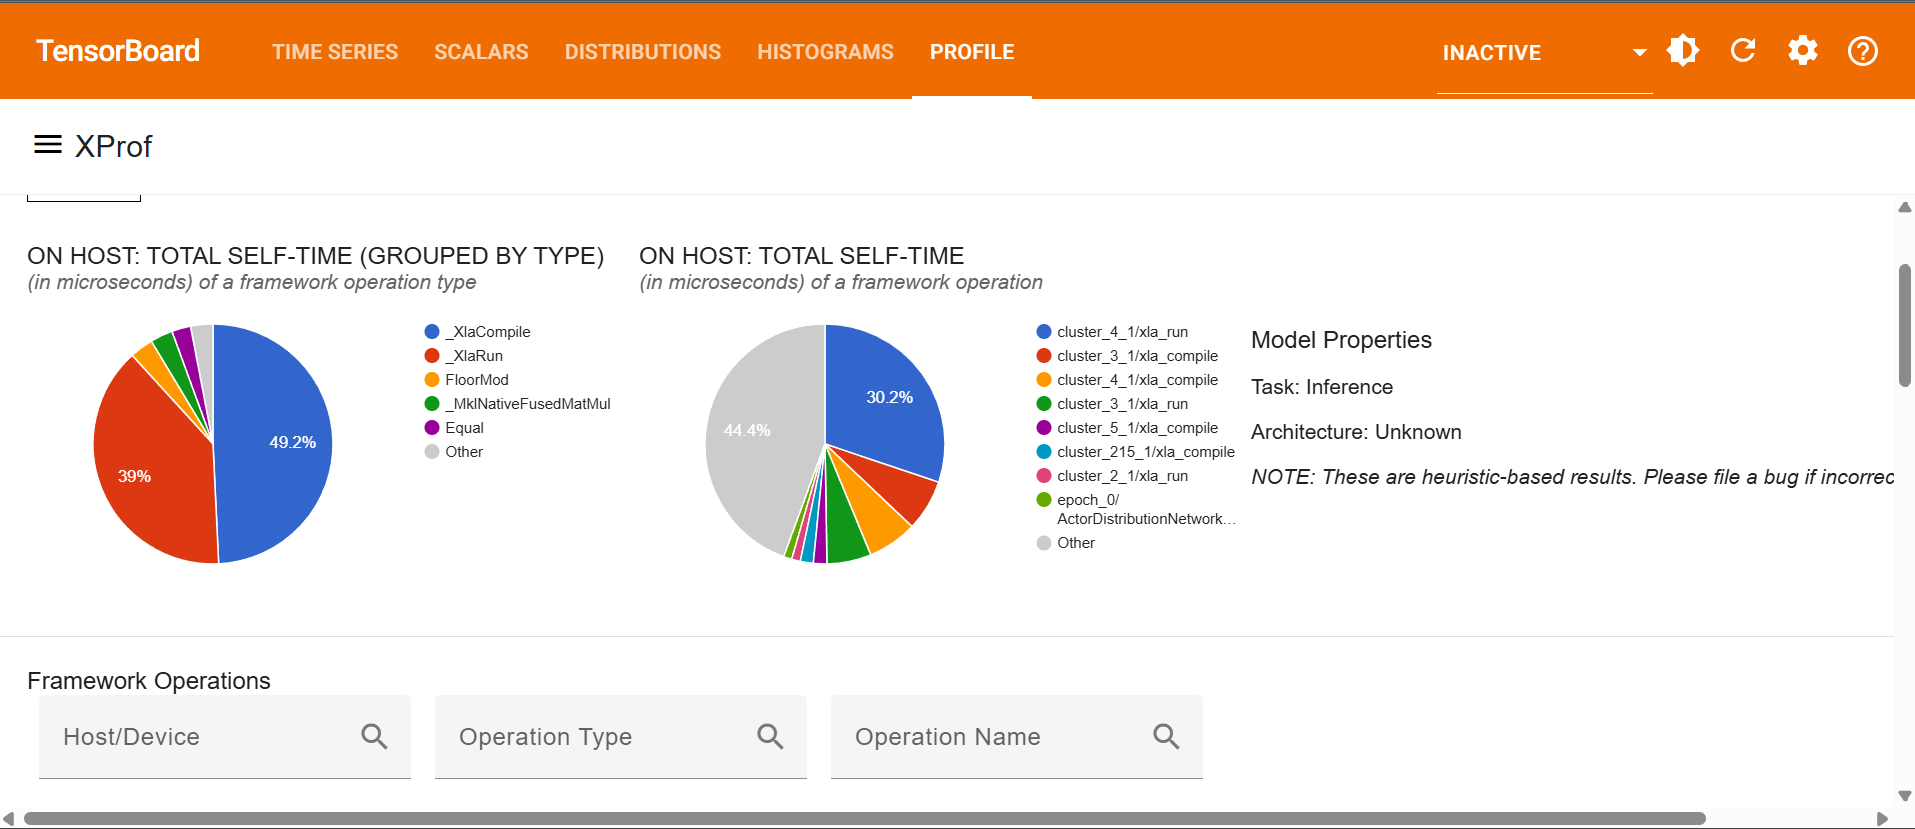
\includegraphics[width=0.85\textwidth]{../pie_chart_execution.png}
\caption{XLA Compilation time breakdown within the training step. The majority of time is spent in compiled XLA kernels.}
\end{figure}

The training throughput was observed at approximately 250--275 steps/second during the training phase (when collecting is not happening), and approximately 15--20 steps/second during the collect+train iteration due to compilation overhead.

\begin{figure}[H]
\centering
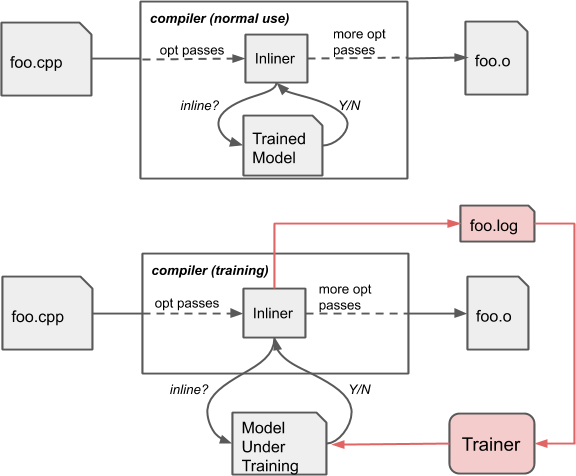
\includegraphics[width=0.85\textwidth]{../rel_vs_dev.png}
\caption{Comparison of original (release) vs refactored (dev) data pipeline. The refactored pipeline eliminates \texttt{Iterator::Root::Prefetch} overhead.}
\end{figure}

\begin{figure}[H]
\centering
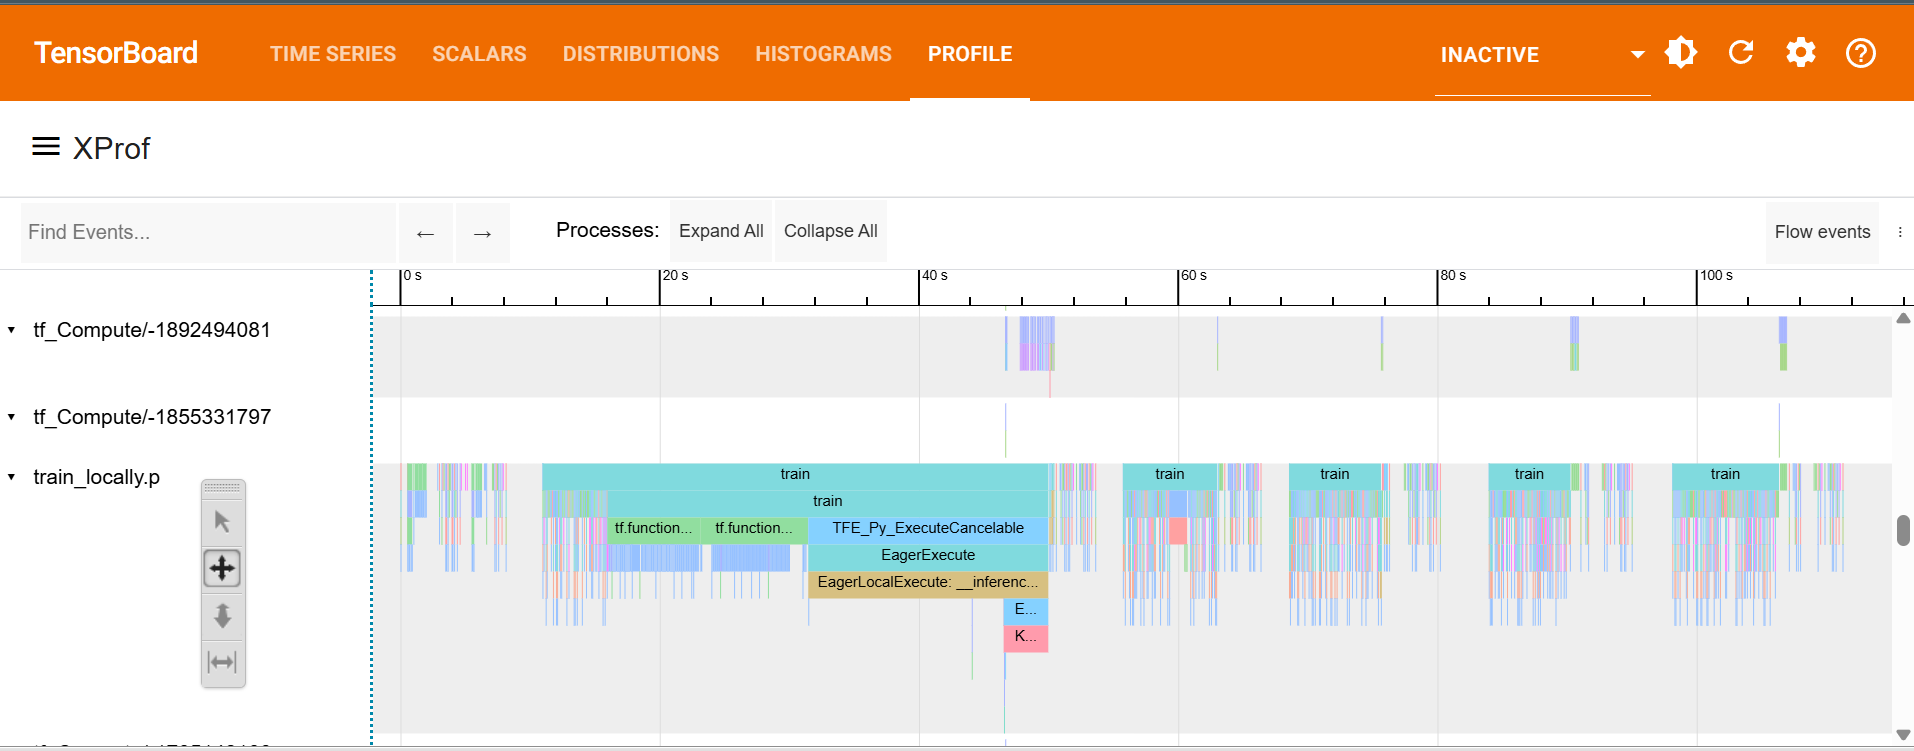
\includegraphics[width=\textwidth]{../tensorboard_trace.png}
\caption{TensorFlow Profiler trace of the training step. Each horizontal band is a CPU thread. The wide dark bands show \texttt{agent.train()} kernel launches; narrow bands correspond to data loading and reward normalization. The bottleneck has shifted to compute (kernel launch).}
\end{figure}

\subsection{Interpretation}

The profiling data reveals that the bottleneck has successfully shifted from data loading to compute. With the original pipeline, approximately 18\% of step time was spent in \texttt{Iterator::Root::Prefetch}---pure TF op dispatch overhead with no useful computation. After the changes, data loading accounts for $\sim$13\% of step time, and the vast majority ($\sim$87\%) is spent in the actual training step (matrix multiplications, gradient computation, optimization).

The XLA JIT auto-clustering fuses small TensorFlow operations into larger compiled kernels. This reduces op dispatch overhead and enables better cache utilization through kernel fusion. The multi-threaded Eigen backend then parallelizes matrix multiplication across CPU cores.

Loss values during a representative training run (from an earlier session with the older pipeline) showed convergence from approximately 0.26 to 0.07 over 6,000 steps. However, comparing loss convergence rates between the old and new pipelines was confounded by the changed hyperparameters (batch size, sequence length, number of modules); the primary metric of interest was throughput, not convergence quality.

One set of training runs illustrated the need for the XLA flags fix: runs without proper \texttt{xla\_cpu\_multi\_thread\_eigen} showed identical step times regardless of batch size, suggesting that matrix operations were serialized. After the fix, increasing batch size showed the expected sub-linear scaling in step time.

\subsection{Limitations}

The evaluation has several limitations. First, the training runs were executed on a shared cluster with varying resource availability, so timing measurements have uncontrolled noise. Second, only the inlining-for-size task was evaluated; the register allocation task may exhibit different performance characteristics. Third, the hyperparameters were tuned for this specific corpus (Fuchsia) and hardware; different setups would likely require re-tuning.

\section{Time Spent on Project}

Based on commit history, batch logs, and notes, the following is an approximate breakdown of time spent:

\begin{table}[H]
\centering
\caption{Time breakdown across major project categories. Total: approximately 30 hours.}
\begin{tabular}{lrr}
\toprule
Category & Hours & Percentage \\
\midrule
Data Pipeline R\&D       & 10 & 34\% \\
XLA JIT Integration      &  5 & 18\% \\
Hyperparameter Tuning    &  4 & 12\% \\
Profiling and Instrumentation & 5 & 16\% \\
Setup and Infrastructure &  4 & 12\% \\
Report and Documentation &  2 &  8\% \\
\midrule
Total & 30 & 100\% \\
\bottomrule
\end{tabular}
\end{table}

\begin{table}[H]
\centering
\caption{Time Spent by Category}
\begin{tabular}{lp{3cm}r}
\toprule
Category & Activities & Hours \\
\midrule
Data Pipeline R\&D & TF profiling, generator rewrite, buffer tuning, test updates & 10 \\
XLA JIT Integration & Env flag setup, multi-thread Eigen, flag fix iteration & 5 \\
Hyperparameter Tuning & Batch size, sequence length, module count experiments & 4 \\
Profiling \& Instrumentation & Perf counters, TF profiler, signal handlers, analysis & 5 \\
Setup \& Infrastructure & LLVM build with MLGO, Fuchsia corpus, Slurm scripts & 4 \\
Report \& Documentation & Presentation, final report writing & 2 \\
\midrule
\textbf{Total} & & \textbf{30} \\
\bottomrule
\end{tabular}
\end{table}

\section{Discussion}

The primary finding is that TensorFlow's \texttt{tf.data} pipeline, while powerful for large-scale distributed data loading, introduces significant overhead when used with in-memory data of modest size. For the MLGO training loop, where all trajectory data fits in memory after one iteration of collection, a simple Python generator is more efficient. This is a case where a lower-level abstraction outperforms a more general but heavier framework.

The XLA JIT integration was surprisingly nuanced. While enabling \texttt{tf\_xla\_cpu\_global\_jit} is well-documented, the interaction between \texttt{TF\_XLA\_FLAGS} and \texttt{XLA\_FLAGS} (and which flags belong in which) is not. The \texttt{xla\_cpu\_multi\_thread\_eigen} flag is particularly important because without it, Eigen operations fall back to a single-threaded implementation, negating the parallelism benefits of modern multi-core CPUs.

The per-step performance counters proved valuable for identifying remaining bottlenecks. Before instrumentation, it was unclear whether data loading, reward computation, or gradient computation dominated step time. After adding counters, it became clear that data loading was the initial bottleneck (commit 1 target), and after fixing that, compute became the dominant term.

\section{Conclusion}

This project successfully optimized the MLGO training loop through three concrete improvements: (1) replacing the \texttt{tf.data} pipeline with a Python generator to eliminate TF op dispatch overhead, (2) enabling XLA CPU JIT compilation with multi-threaded Eigen for parallel matrix operations, and (3) adding performance instrumentation for data-driven optimization targeting. The result is a training loop where $\sim$87\% of step time is spent on actual computation rather than data pipeline overhead.

\section{Next Steps}

Future work could include:

\begin{itemize}
    \item \textbf{Profile-guided tuning}: Use TF profiler traces (now being collected) to identify remaining bottlenecks within the training step itself.
    \item \textbf{XLA compilation cache tuning}: Monitor the \texttt{xla\_dump\_max\_hlo\_modules} hit rate and adjust the cache size to minimize recompilation.
    \item \textbf{Generator vs tf.data at scale}: Evaluate whether the generator path remains beneficial at much larger \texttt{num\_modules} scales (e.g., thousands of modules), where lazy loading may become advantageous again.
    \item \textbf{Multi-GPU training}: Test XLA flag compatibility with GPU training, as XLA JIT behavior differs on GPU versus CPU.
\end{itemize}

\begin{thebibliography}{9}
\bibitem{mlgo2021}
Trofin, M., Qian, Y., Brevdo, E., Lin, Z., Choromanski, K., \& Li, X. D. (2021).
\emph{MLGO: a Machine Learning Guided Compiler Optimizations Framework}.
arXiv preprint arXiv:2101.04808.

\bibitem{google-mlgo}
Google. \emph{ml-compiler-opt: Infrastructure for Machine Learning Guided Optimization in LLVM}.
\url{https://github.com/google/ml-compiler-opt}

\bibitem{schulman2017}
Schulman, J., Wolski, F., Dhariwal, P., Radford, A., \& Klimov, O. (2017).
\emph{Proximal Policy Optimization Algorithms}. arXiv preprint arXiv:1707.06347.

\bibitem{xla}
TensorFlow. \emph{XLA: Optimizing Compiler for Machine Learning}.
\url{https://www.tensorflow.org/xla}
\end{thebibliography}

\end{document}
